\newpage
\section{Auswertung}
\label{sec:Auswertung}
\subsection{Fehlerrechnung}
Für die Fehlerrechnung wurde die Gaußsche Fehlerfortplanzung
\begin{equation}
\Delta f=\sqrt{\left(\frac{\partial f}{\partial x}\right)^2(\Delta x)^2+\left(\frac{\partial f}{\partial y}\right)^2(\Delta y)^2+...+\left(\frac{\partial f}{\partial z}\right)^2(\Delta z)^2}
\end{equation}
für fehlerbehaftete Werte $x,y,...,z$ mit den Unsicherheiten $\Delta x,\Delta y,..,\Delta z$ sowie der Fehler des Mittelwertes:
\begin{equation}
\Delta \bar{x}=\sqrt{\frac{1}{N(N-1)}\sum_{k=1}^N(x_k-\bar{x})^2}
\end{equation}
mit dem Mittelwert $\bar{x}$ verwendet.
\subsection{Invertierender Verstärker}
Für den Invertierenden Verstärker wurden die Amplitude und die Phasenverschiebung $\Phi$ der Amplitude der Ausgangsspannung $U_A$ in Abhängigkeit von der Frequenz $f$ gemessen. Eine solche Messung wurde mit drei verschiedenen Konfigurationen von Wiederständen ausgeführt.

Mittels der Eingangsamplitude des Signalgenerators wurde für alle Messungen aus den gemessenen Amplituden jeweils die Verstärkung $G$ bestimmt und anschließend in einem doppellogarithmischen Koordinatensystem in Abhängigkeit von der Frequenz abgebildet. 
\begin{figure}
\centering
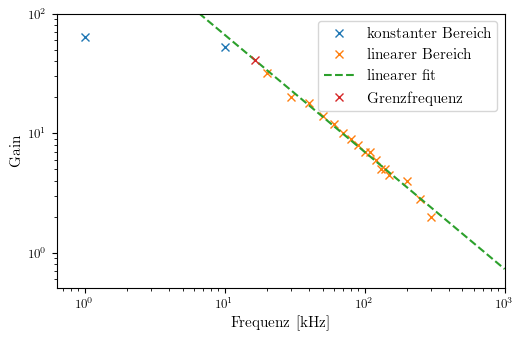
\includegraphics[width=0.6\textwidth]{Frequenzgang Messreihe1}
\label{fig:invert freq 1}
\caption{Verstärkung in Abhängigkeit von der Frequenz in doppellogarithmischer Darstellung für einen invertierten Verstärker mit Wiederständen $R_1=\SI{1}{\kilo\ohm}$ und $R_2=\SI{68}{\kilo\ohm}$}
\end{figure}
\begin{figure}
\centering
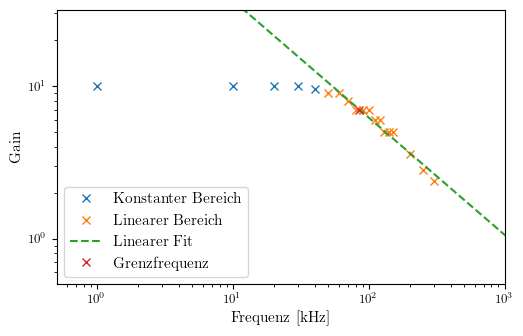
\includegraphics[width=0.6\textwidth]{Frequenzgang Messreihe2}
\label{fig:invert freq 2}
\caption{Verstärkung in Abhängigkeit von der Frequenz in doppellogarithmischer Darstellung für einen invertierten Verstärker mit Wiederständen $R_1=\SI{10}{\kilo\ohm}$ und $R_2=\SI{100}{\kilo\ohm}$}
\end{figure}
\begin{figure}
\centering
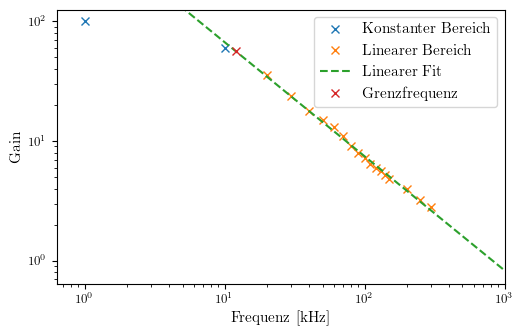
\includegraphics[width=0.6\textwidth]{Frequenzgang Messreihe3}
\label{fig:invert freq 3}
\caption{Verstärkung in Abhängigkeit von der Frequenz in doppellogarithmischer Darstellung für einen invertierten Verstärker mit Wiederständen $R_1=\SI{1}{\kilo\ohm}$ und $R_2=\SI{100}{\kilo\ohm}$}
\end{figure}
\begin{figure}
\centering
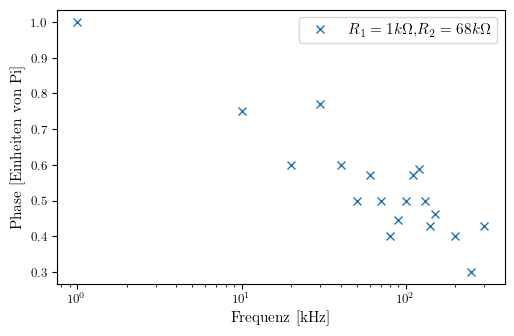
\includegraphics[width=0.6\textwidth]{Operationsverstärker Phase1}
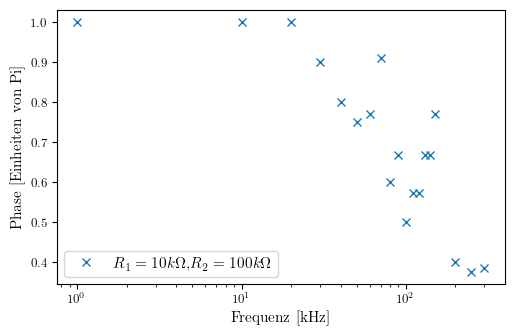
\includegraphics[width=0.6\textwidth]{Operationsverstärker Phase2}
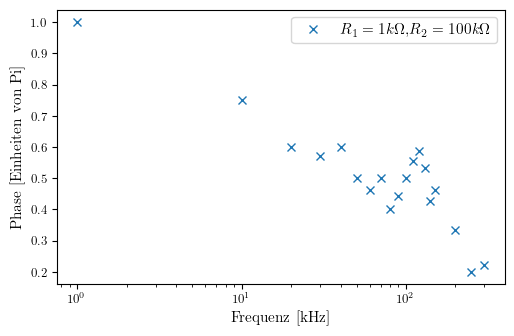
\includegraphics[width=0.6\textwidth]{Operationsverstärker Phase3}
\label{fig:invert freq Ph}
\caption{Phasenverschiebung in Einheiten von $\pi$ Abhängigkeit von der Frequenz in halblogarithmischer Darstellung für einen invertierten Verstärker für alle die drei vorgenommenen Messreihen.}
\end{figure}
Die Ergebnisse sind in den Abbildungen $\ref{fig:invert freq 1}$, $\ref{fig:invert freq 2}$, $\ref{fig:invert freq 3}$ dargestellt. Die Phasenverschiebungen der drei Messreihen finden sich in Abbildung 
Im Bereich des linearen Zusammenhangs zwischen beiden Größen kann ein Fit der Form:
\begin{equation}
\log(G)=m\log(f)+b
\end{equation}
welche im nicht logarithmischen Raum einer Funktion der Form:
\begin{equation}
G(f)=Bf^m
\end{equation}
entspricht. Für die drei Messreihen lauten die Fitfunktionen:
\begin{gather}
G_1(f)=(634,79\pm76,14)f^{-0,98\pm0,26} \\
G_2(f)=(157,25\pm36,32)f^{-0,71\pm0,05} \\
G_3(f)=(605.03\pm63,597)f^{-0,95\pm0,02}
\end{gather}
Die annähernd konstante Verstärkung im niederfrequenteren Bereich $G_c$ kann durch den Mittelwert der entsprechenden Messpunkte ermittelt werden. Mithilfe dieses Wertes sowie der gefitteten Funktionen im linearen Bereich kann die Grenzfrequenz $f_g$ bestimmt werden. Diese ist definiert als die Frequenz, bei der die konstante Verstärkung sich um 3 dB bzw. den Faktor $1/\sqrt{2}$ verringert hat. Die Grenzfrequenz kann gemäß der gefitteten Funktion durch die Formel
\begin{equation}
f_g=\left(\frac{V_c}{B\sqrt{2}}\right)^m
\end{equation}
Die Wiederstände der Messreihen sowie die berechneten Verstärkungen und Grenzfrequenzen lauten:
\begin{align*}
    &\text{Messung 1:}\\
    & R_1 = \SI{1}{\kilo\ohm}     &&  R_2 = \SI{68}{\kilo\ohm}     &&  G_c = 58\pm6  && f_g=\SI{16,4\pm2,3}{\kilo\hertz}  \\
    &\text{Messung 2:}\\
   & R_1 = \SI{10}{\kilo\ohm}     &&  R_2 = \SI{100}{\kilo\ohm}     &&  G_c = 9,9\pm0,1  && f_g=\SI{85\pm33}{\kilo\hertz} \\
    &\text{Messung 3:}\\
   & R_1 = \SI{1}{\kilo\ohm}     &&  R_2 = \SI{100}{\kilo\ohm}     &&  G_c = 80\pm20  && f_g=\SI{12\pm3,5}{\kilo\hertz} \\
\end{align*}
\subsection{Integrator}
Für den Integrator wurden ein Wiederstand von $R=\SI{10}{\kilo\ohm}$ und ein Kondensator mit der Kapazität von $C=\SI{100}{\nano\farad}$ verwendet.
\begin{figure}
\centering
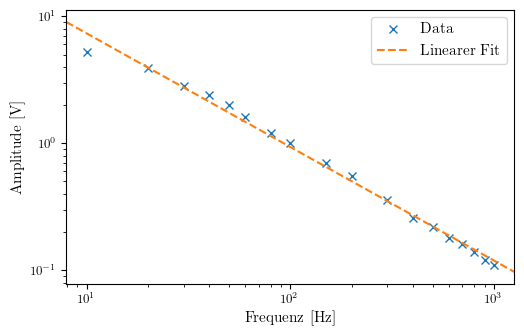
\includegraphics[width=0.6\textwidth]{Integrator}
\label{fig:int}
\caption{Amplitude in Abhängigkeit von der Frequenz in doppellogarithmischer Darstellung für einen integrator mit Widerstand $R=\SI{10}{\kilo\ohm}$ und Kapazität $C=\SI{100}{\nano\farad}$}
\end{figure}
\begin{figure}
\centering
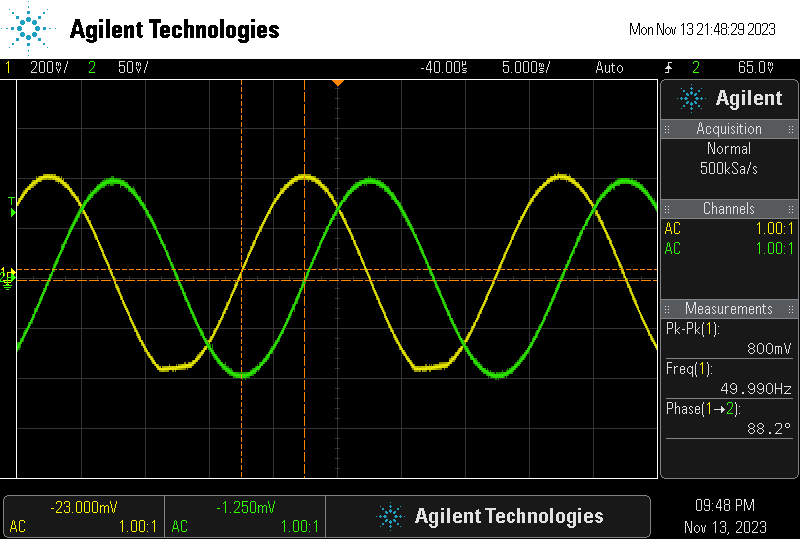
\includegraphics[width=0.6\textwidth]{scope_3}
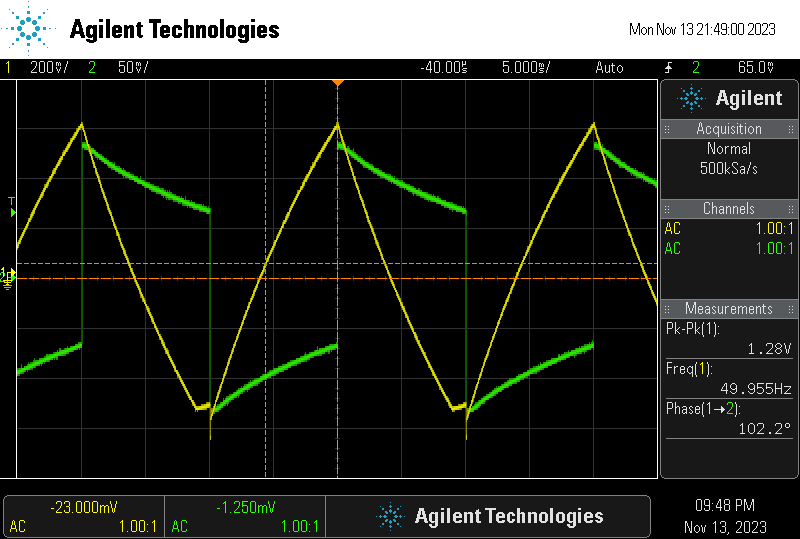
\includegraphics[width=0.6\textwidth]{scope_4}
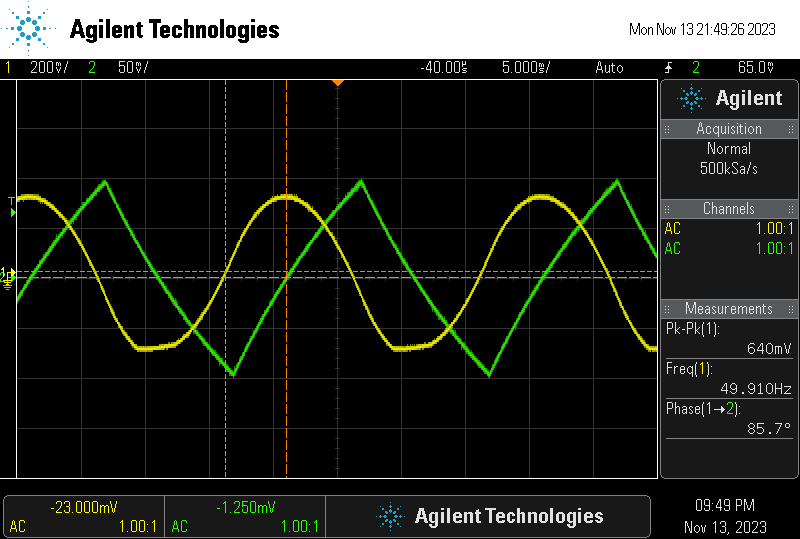
\includegraphics[width=0.6\textwidth]{scope_5}
\label{fig:int screenshots}
\caption{Ausgangssignal eines Integrators (gelb) für Sinus-, Rechteck und Dreicksspannungen als Eingangssignal (grün)}
\end{figure}
Abbildung $\ref{fig:int}$ zeigt die Amplitude der Ausgangsspannung in Abhängigkeit von der Frequenz. Zusätzlich ist eine Fitfunktion:
\begin{equation}
U_{int}(f)=(57,52\pm5,7)f^{-0,89\pm0,19}
\end{equation}
angelegt. Ein solcher Verlauf entspricht der Erwartung für den Verstärkungsverlauf eines Integrators.
Die Bilder in Abbildung $\ref{fig:int screenshots}$ des zeigen das Ausgangssignal des Integrators für verschiedene Eingangsspannungen. Wie zu erwarten ergibt sich aus einem Sinussignal nach Integration ein Cosinussignal, aus einer Rechteckspannung eine Dreieckspannung und aus einer Dreieckspannung ein Parabolischer Verlauf.
\subsection{Differentiator}
Der Differentiator verwendet einen Widerstand von $R=\SI{100}{\kilo\ohm}$ und eine Kapazität von $C=\SI{22}{\nano\farad}$.
\begin{figure}
\centering
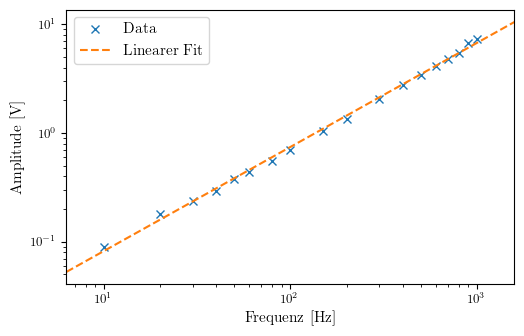
\includegraphics[width=0.6\textwidth]{Differentiator}
\label{fig:diff}
\caption{Amplitude in Abhängigkeit von der Frequenz in doppellogarithmischer Darstellung für einen Differentiator mit Widerstand $R=\SI{100}{\kilo\ohm}$ und Kapazität $C=\SI{22}{\nano\farad}$}
\end{figure}
\begin{figure}
\centering
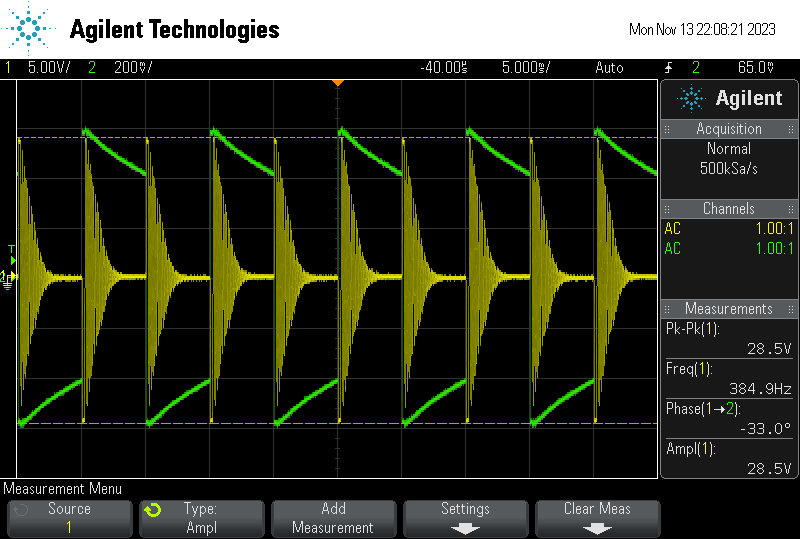
\includegraphics[width=0.6\textwidth]{scope_6}
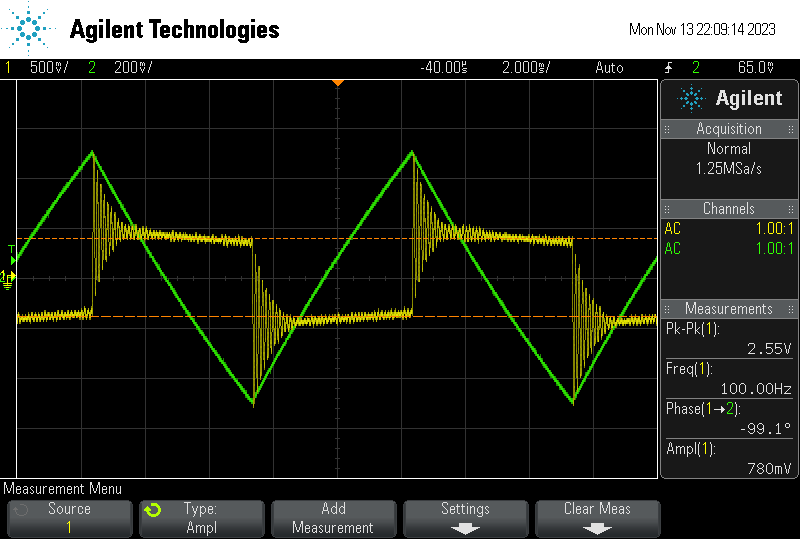
\includegraphics[width=0.6\textwidth]{scope_9}
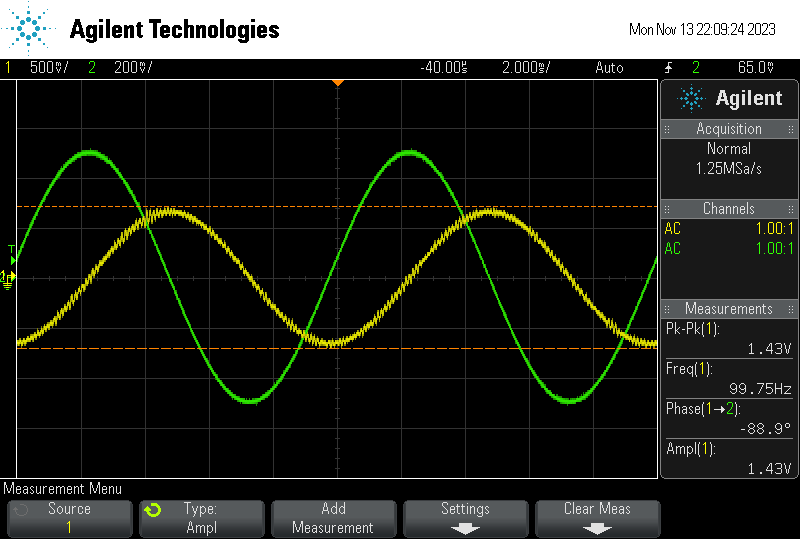
\includegraphics[width=0.6\textwidth]{scope_10}
\label{fig:diff screenshots}
\caption{Ausgangssignal eines Differentiators (gelb) für Sinus-, Rechteck und Dreicksspannungen als Eingangssignal (grün)}
\end{figure}
Die Amplitude des Ausgangssignals in Abhängigkeit von der Frequenz findet sich in Abbildung $\ref{fig:diff}$. Der zugehörige Fit lautet:
\begin{equation}
U_{diff}(f)=(0,009\pm0.000,5)f^{0,96\pm0,01}
\end{equation}
Wie zu erwarten steigt die Amplitude bzw. die Verstärkung mit steigender Frequenz an, wie sich auch im Fit zeigt.
Wie beim Integrator wird auch beim Differentiator durch die Fotos ($\ref{fig:diff screenshots}$) die Reaktion auf die unterschiedlichen Eingangssignale veranschaulicht. Das Ausgangssignal erwartungsgemäß die Ableitung der jeweilligen Eingangsfunktion.
\subsection{Schmitt Triger}
Für den Schmitt Triger wurden die Widerstände $R_1=\SI{10}{\kilo\ohm}$ und $R_2=\SI{100}{\kilo\ohm}$ sowie die Betriebsspannungen $U_{\pm}=\pm\SI{15}{\volt}$ verwendet.
Somit ergeben sich die theoretischen Kippspannungen zu:
\begin{equation}
U_{kipp,\pm}=U_{\pm}\frac{R_1}{R_2}=\pm\SI{1,5}{\volt}
\end{equation}
Durch variiren der Amplitude des Eingangssignals konnte der Kippunkt und somit der Betrag der Kippspannung zu $U_{kipp}=\SI{1,465}{\volt}$ ermittelt werden. Weiterhin wurden durch Anlegen einer Dreieckspannung an jeweils drei Punkten der Kippunkt der Ausgangsspannung am Oszilloskop beobachtet. Durch Bildung der Mittelwerte führt dies zu den Kippspannungen:
\begin{gather}
U_{kipp,+}=\SI{1,567\pm0,06}{\volt} \\
U_{kipp,-}=\SI{1,5\pm0,058}{\volt}
\end{gather}
\subsection{Generator}
Für die Konstruktion des Generators wurden die Widerstände $R_1=\SI{10}{\kilo\ohm}$, $R_2=\SI{100}{\kilo\ohm}$ und $R_3=\SI{1}{\kilo\ohm}$ sowie die Kapazität $C=\SI{e-6}{\farad}$ verwendet. Dies liefert eine theoretische Frequenz des Ausgangssignals von:
\begin{equation}
f_a=\frac{R_2}{4CR_1R_3}=\SI{2,5}{\kilo\hertz}
\end{equation}
sowie eine Amplitude von
\begin{equation}
U_a=U_{max}\frac{R_1}{R_2}=\SI{1,4}{\kilo\hertz}
\end{equation}
\begin{figure}
\centering
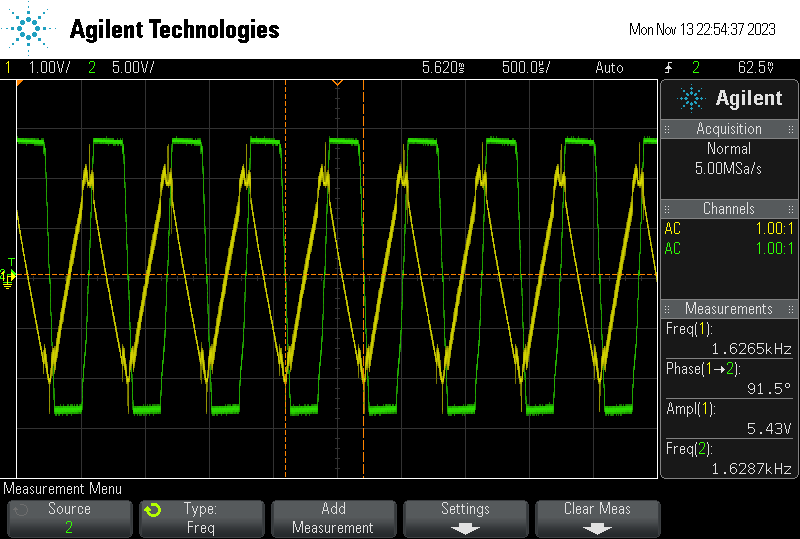
\includegraphics[width=0.6\textwidth]{scope_14}
\label{fig:Gen screenshots}
\caption{Dreiecksschwingung und Rechteckschwingung des Generators}
\end{figure}
Die experimentellen Werte der Generierten Ausgangsspannung $f_{a,exp}=\SI{1,62}{\kilo\hertz}$, $U_{a,exp}=\SI{2,1}{\volt}$ lassen sich der Abbildung $\ref{fig:Gen screenshots}$ entnehmen. 
\subsection{Gedämpfte Schwingung}
Für die gedämpfte Schaltung wurde eine Schaltung mit den Kenndaten $R=\SI{1}{\kilo\ohm}$ und $C=\SI{100}{\nano\farad}$ verwendet.
\begin{figure}
\centering
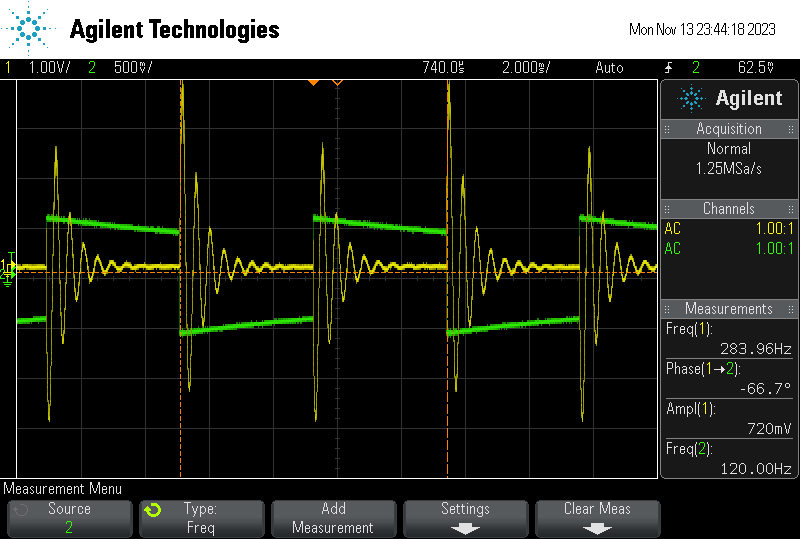
\includegraphics[width=0.6\textwidth]{scope_15}
\label{fig:ged screenshots}
\caption{Ausgangssignal eines Integrators (gelb) für Sinus-, Rechteck und Dreicksspannungen als Eingangssignal (grün)}
\end{figure}
Die resultierende gedämpfte Schwingung ist in Abbildung $\ref{fig:ged screenshots}$ zu sehen. Die theoretische Periodendauer lässt sich damit durch die Formel
\begin{equation}
T_{theo}=2\pi RC=\SI{628,3}{\micro\second}
\end{equation}
berechnen. Um die Periodendauer sowie die Abklingzeit $\tau$ zu berechnen wird eine der Schwingungen ausgewählt und ein exponentieller Fit an die Maxima angelegt um die einhüllende zu bestimmen.
\begin{figure}
\centering
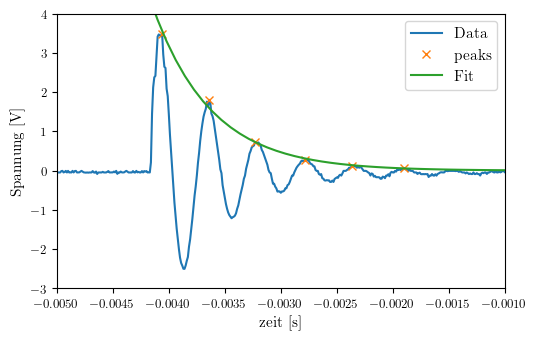
\includegraphics[width=0.49\textwidth]{ged schwing}
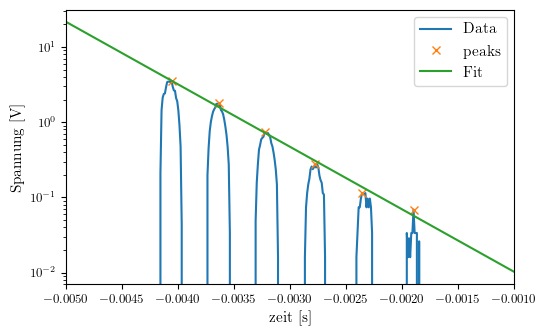
\includegraphics[width=0.49\textwidth]{ged schwing log}
\label{fig:ged schwing}
\caption{Amplitude in Abhängigkeit von der Zeit für eine gedämpfte Schwingung in regulärer und halblogarithmischer Darstellung}
\end{figure}
Das Ergebniss findet sich in Abbildung $\ref{fig:ged schwing}$. Die zugehörige Fitfunktion lautet:
\begin{equation}
U_{schwing}(t)=a\exp(-mt)=(0,015\pm0,0004)\exp(-(1912,84\pm86,98)t)
\end{equation}
woraus die Abklingzeit
\begin{equation}
\tau=1/m=\SI{523\pm23,8}{\micro\second}
\end{equation}
bestimmt werden kann. Weiterhin kann durch die mittlere Distanz zwischen den Maxima die Periodendauer bestimmt werden:
\begin{equation}
T_{exp}=\SI{432\pm9,7}{\micro\second}
\end{equation}
